\documentclass{article}

\usepackage[
  paperheight=8.5in,
  paperwidth=5.5in,
  left=10mm,
  right=10mm,
  top=20mm,
  bottom=20mm]{geometry}
\usepackage[utf8]{inputenc}

\usepackage{graphicx}
\usepackage{wrapfig}
\usepackage[bottom]{footmisc}
\usepackage{listings}
\usepackage{enumitem}

\usepackage{wrapfig}
\usepackage{ragged2e}

\usepackage{array}
\usepackage[table]{xcolor}
\usepackage{multirow}
\usepackage{booktabs}
\usepackage{hhline}
\definecolor{palegreen}{rgb}{0.6,0.98,0.6}

\usepackage{amsmath}
\usepackage{amssymb}
\usepackage{multicol}
\usepackage{lipsum}
\usepackage{hyphenat}
\PassOptionsToPackage{hyphens}{url}
\usepackage{url}

\usepackage{rotating}

%\usepackage{xeCJK}

%% support use of straight quotes in code listings
\usepackage[T1]{fontenc}
\usepackage{textcomp}
\usepackage{listings}
\lstset{upquote=true}

%% for shrinking space between lines
\usepackage{setspace}

\newcommand*{\affaddr}[1]{#1} % No op here. Customize it for different styles.
\newcommand*{\affmark}[1][*]{\textsuperscript{#1}}
\newcommand*{\email}[1]{\small{\texttt{#1}}}
\newcommand{\tarot}{\textsc{Tarot}}
\renewcommand*\contentsname{\centering Table of Contents}

\renewcommand{\footnoterule}{%
  \kern -3pt
  \hrule width \textwidth height 0.5pt
  \kern 2pt
}

% remove date
\date{}

\usepackage{titlesec}
\titleformat*{\section}{\large\bfseries}
\titleformat*{\subsection}{\normalsize\bfseries}
\titleformat*{\subsubsection}{\normalsize\bfseries}

\usepackage{biblatex}


\usepackage{algorithm}
\usepackage{algpseudocode}

\addbibresource{zeichickSW24.bib}

\title{Confidence and Competence: The Impact of National Cyber League Participation on Career Development in Cybersecurity\footnote{\protectCopyright \copyright 2024 by the Consortium for Computing Sciences in Colleges.
Permission to copy without fee all or part of this material is granted provided
that the copies are not made or distributed for direct commercial advantage,
the CCSC copyright notice and the title of the publication and its date appear,
and notice is given that copying is by permission of the Consortium for
Computing Sciences in Colleges.  To copy otherwise, or to republish, requires
a fee and/or specific permission.
}
}

\author{
David Zeichick \\
Computer Science\\
California State University, Chico\\
Chico, CA 95929\\
\email{dzeichick@csuchico.edu}\\
}

\begin{document}
\maketitle
\thispagestyle{empty}
\pagestyle{empty}

\begin{abstract}
This study investigates the career impacts of participating in the National Cyber League (NCL) cybersecurity competition. It assesses the effect of such competitive experiences on job interview opportunities, interview performance, and the practical application of skills learned in the competition to professional roles. Data was collected through a survey of NCL participants. Results indicate a significant link between participation in the NCL and increased confidence in cybersecurity abilities through hands-on experience which was noted to be absent in their formal education. Furthermore, the competition served as an incentive for further learning in the field of cybersecurity.
\end{abstract}

\section{Introduction and Related work}

Cybersecurity competitions have been recognized for their pedagogical benefits, engaging learners, and providing hands-on experiences\cite{chothia2015offline,katsantonis2017conceptual,de2018adles}. Participants in cybersecurity competitions report increased motivation, better understanding of professional requirements, and enhanced teamwork skills through cooperation on team based competitions\cite{3gse15,dark2014advancing,vigna2014ten}. Furthermore, these competitions foster improved collaboration abilities as participants work together in team-oriented challenges\cite{gotel2009global}. 

Despite cybersecurity competitions existence of over two decades and the growing popularity of them, the existing body of research has not extensively explored cybersecurity competitions from the viewpoint of cybersecurity professionals already in the field\cite{chothia2015offline}. Moreover, there is a scarcity of research comparing the skills demanded in cybersecurity positions with those imparted through participation in such competitions\cite{soups16}.

To address this gap, Wee et al.\cite{soups16} investigated the alignment between the skills demanded by the cybersecurity workforce and those honed through cybersecurity competitions. Their research centered on participants of New York University's Capture the Flag (CTF) event during Cybersecurity Awareness Week (CSAW). Utilizing data from a substantial prior survey, which explored the demographics drawn to cybersecurity and ways to enhance competitions, the study homed in on 89 professionals from the initial 217 respondents who were working in the cybersecurity sector. Analysis of 16 multiple-choice questions from the "much larger survey" revealed that 89.9\% of these professionals placed high value on the skills developed in competitions. Additionally, over half attributed their career choice to these competitions, and 69\% recognized the competitions as potent recruitment channels for the industry\cite{soups16}.


\section{Methods}

This research aimed to determine whether participation in the National Cyber League (NCL) was perceived as beneficial for securing employment in the cybersecurity sector and to what extent the competencies developed during the NCL were applicable to participants' current professional roles. To assess this, the study surveyed NCL participants who are now working in the field of cybersecurity. 

The NCL was selected for its approach to addressing common issues found in some cybersecurity contests. Concerns regarding the depth and focus of some competitions suggest they may not fully prepare participants for the diverse range of skills required in the industry\cite{cheung2012effectiveness,katsantonis2017conceptual,mouheb2019cybersecurity}. Additionally, competitions often lack formal training for entrants\cite{mouheb2019cybersecurity}, presenting a significant barrier as many events necessitate extensive prior knowledge\cite{cheung2012effectiveness}.

The NCL's structure comprises four phases: the Gym, with guided challenges for skill-building; the Practice Game, encouraging collaborative problem-solving; the Individual Game, for personal skill assessment; and the Team Game, where groups of up to seven collaborate\cite{nclwebsite}. Each phase offers a variety of difficulties across nine cybersecurity categories that correspond with the National Institute of Standards and Technology’s (NIST) National Initiative for Cybersecurity Education’s (NICE) work roles. These categories include cryptography, password cracking, log analysis, network traffic analysis, forensics, web application exploitation, scanning, enumeration and exploitation, and open-source intelligence, providing a comprehensive range of skills development and assessment for participants.

To recruit participants for the survey we contacted NCL alumni via two different channels.  First, we utilized LinkedIn to identify individuals who had mentioned NCL in their skills section and held a current position within the cybersecurity field.  We then sent out connection requests on LinkedIn and successfully established connections with 62 professionals. Upon connecting, we sent each individual a direct message on LinkedIn with an invitation to contribute to our research, which read: ``I'm hoping you can take about 10 minutes to help me with some research that I am doing. I'm studying how/if the NCL helped prepare you for your career in cybersecurity.''  The message also included a link to the survey hosted by Survey Monkey. We received completed surveys from 34 individuals in the group, a 55\% response rate.

Next, we partnered with the National Cyber League (NCL) to contact 6,013 of their college graduate alumni, whose expected graduation dates were known from their registration details. Although we were not certain of their actual graduation status or whether they were employed in the cybersecurity sector, we proceeded with the outreach. From this group, we received 47 completed surveys, resulting in a response rate of 0.8\%.

The survey consisted of 35 questions; it included 27 quantitative queries using a Likert scale, five open-ended qualitative inquiries, one binary yes/no question, and two queries for consent to disclose their identity, followed by a prompt for their name and email address. The survey was conducted online via Survey Monkey, with each response's start and end times, as well as their IP address, being logged.


\section{Results and Discussion}

The survey consisted of question on four main topic areas: 1) the influence the NCL had on their interest in cybersecurity, 2) the skills acquired through the NCL, 3) the impact of the NCL on employment, and 4) the relevance of the NCL to their current role. We had a total of 81 responses.

\subsection{Quantitative Results}

Participants largely agreed on the following, as indicated by the distributions skewed towards higher values:
\begin{enumerate}[noitemsep]
\item Motivation to Learn About Cybersecurity: Responses concentrated around high values, indicating a strong agreement on increased motivation (see figure \ref{fig:figure1}). Mean = 4.66, Standard Deviation = 0.62
\item Understanding of Cybersecurity: A skew towards higher ratings suggests a consensus on the NCL's positive impact on understanding cybersecurity (see \ref{fig:figure2}). Mean = 4.49, Standard Deviation = 0.66
\item Hands-On Experience Not Available in Formal Education/Training: The peak at higher values indicates agreement on the value of NCL's hands-on experience (see figure \ref{fig:figure3}). Mean = 4.22, Standard Deviation = 0.86
\item Confidence in Cybersecurity Field: A skew towards higher scores suggests a strong consensus on the NCL enhancing participants' confidence (see figure \ref{fig:figure4}). Mean = 4.22, Standard Deviation = 0.83
\end{enumerate}

\begin{figure}
\centering
\lineskip=-\fboxrule
  \fbox{\begin{minipage}{\dimexpr .47\textwidth-2\fboxsep-2\fboxrule}
  \centering
  \fbox{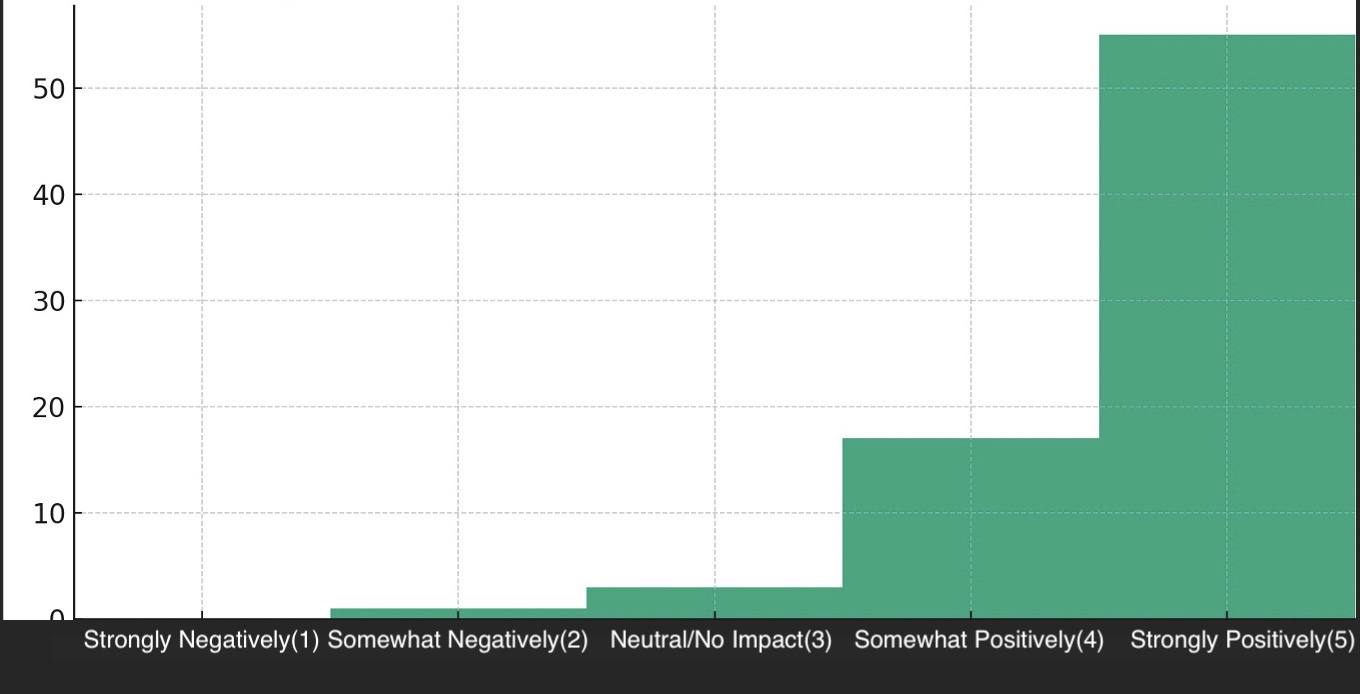
\includegraphics[width=.9\linewidth]{figure1.jpg}}
\caption{To what extent did the NCL impact your motivation to learn more about cybersecurity. either positively or negatively?}
  \label{fig:figure1}
  \end{minipage}} % end minipage AND fbox
  \fbox{\begin{minipage}{\dimexpr .47\textwidth-2\fboxsep-2\fboxrule}
  \centering
  \fbox{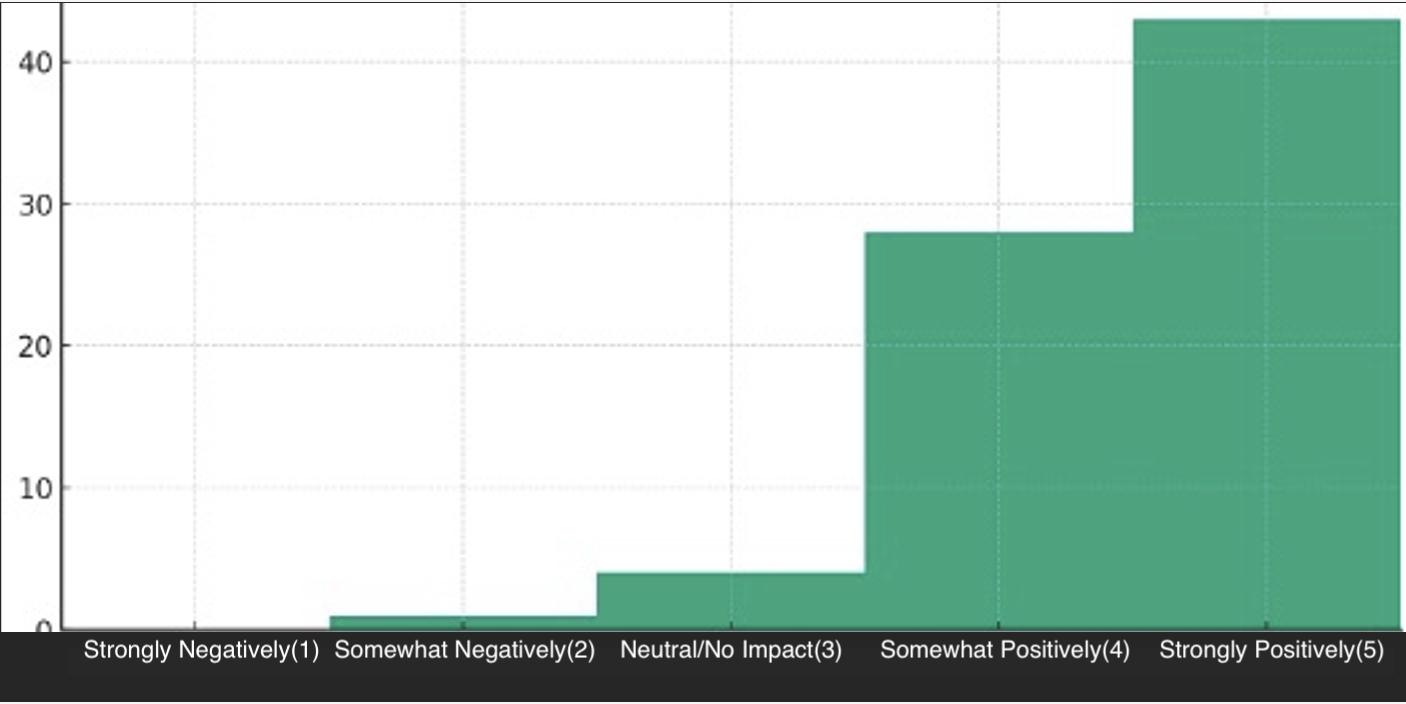
\includegraphics[width=.9\linewidth]{figure2.jpg}}
\caption{To what extent did the NCL influence your understanding of cybersecurity, either positively or negatively?}
  \label{fig:figure2}
\end{minipage}} % end minipage AND fbox
\end{figure}

\begin{figure}
\centering
  \fbox{\begin{minipage}{\dimexpr .47\textwidth-2\fboxsep-2\fboxrule}
  \centering
  \fbox{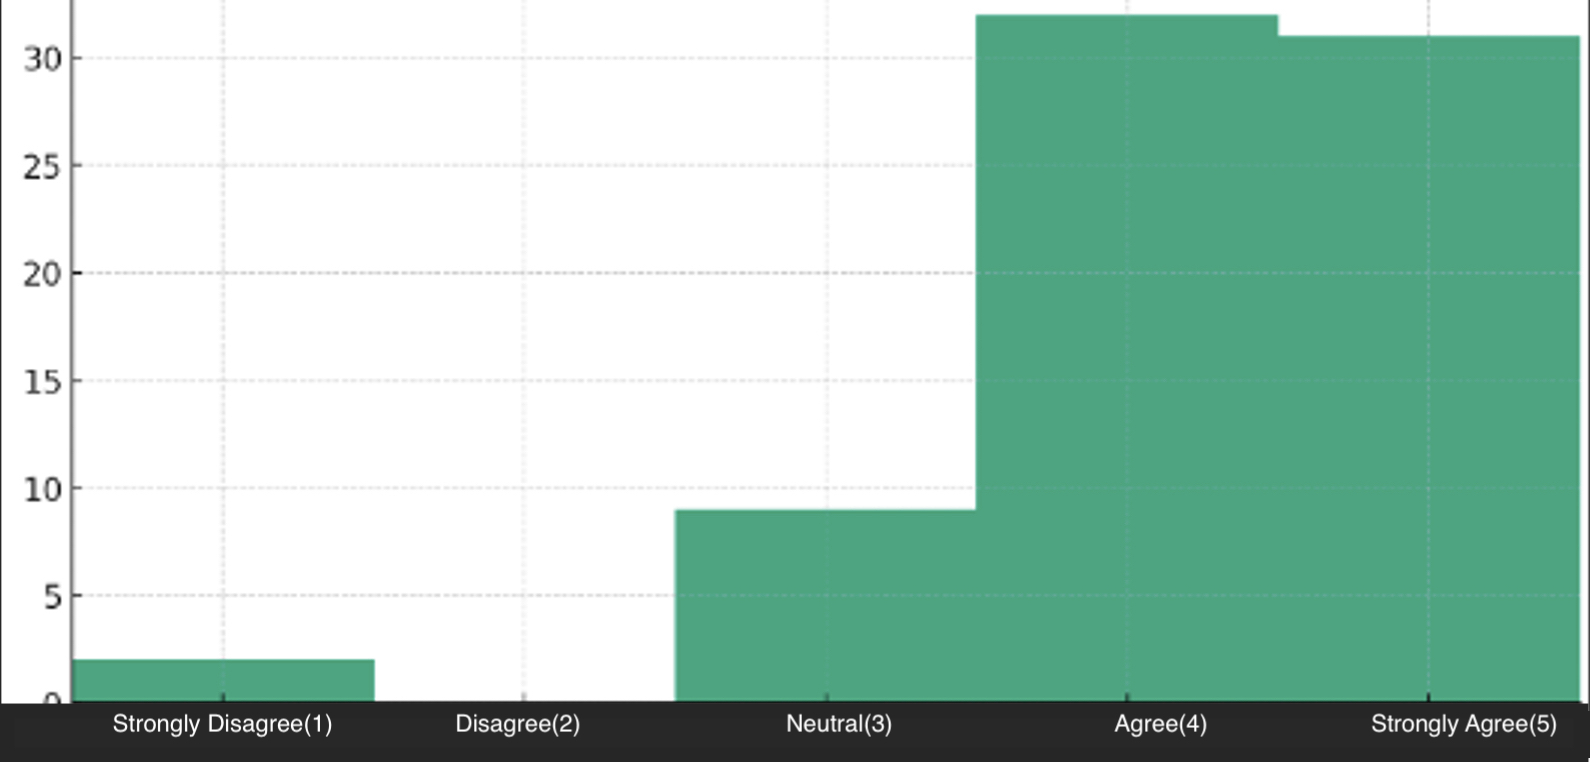
\includegraphics[width=.9\linewidth]{figure3.jpg}}
\caption{The NCL provided hands-on experience that was not available in my formal education or training.}
  \label{fig:figure3}
\end{minipage}}
  \fbox{\begin{minipage}{\dimexpr .47\textwidth-2\fboxsep-2\fboxrule}
  \centering
  \fbox{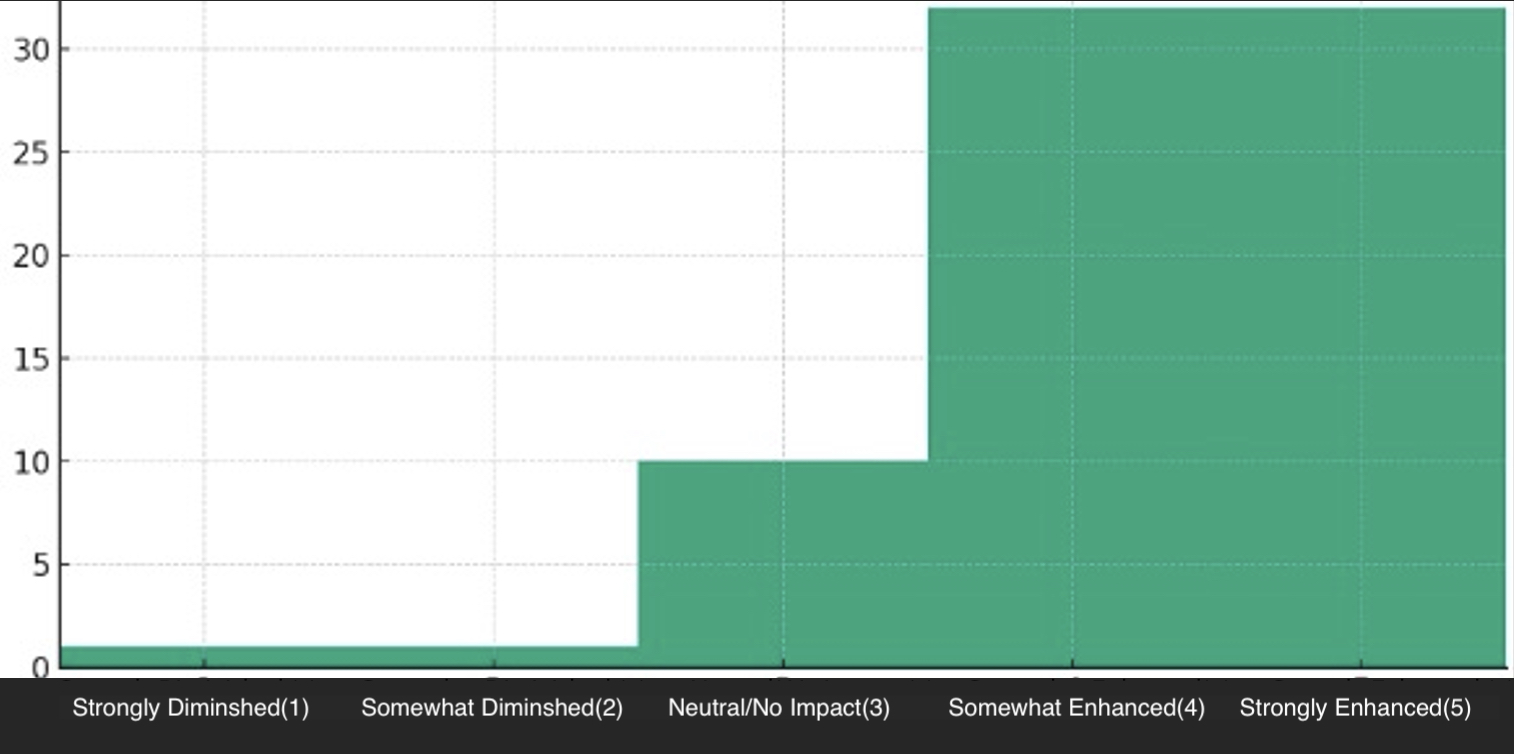
\includegraphics[width=.9\linewidth]{figure4.jpg}}
\caption{To what extent did the NCL affect your confidence in the cybersecurity field, either positively or negatively?}
  \label{fig:figure4}
\end{minipage}}
\end{figure}

Participants had more varied opinions on the following, as indicated by more evenly distributed responses or lack of a strong single peak. For the question about the NCL being discussed during the job interview, the responses were more spread out, indicating varied experiences regarding the discussion of NCL in job interviews (42.31\% yes and 57.69\% no). When asked about encountering similar problem in their current job, the distribution suggests varied experiences about encountering NCL-like problems in current jobs (see figure \ref{fig:figure5}). Responses were also distributed for the question about real-world relevance of NCL challenges, reflecting varied opinions on how closely NCL activities mirror real-world scenarios (see figure \ref{fig:figure6}). The rest of the quantitative questions are listed below in figure \ref{fig:figure7}.

\begin{figure}
\centering
  \fbox{\begin{minipage}{\dimexpr .47\textwidth-2\fboxsep-2\fboxrule}
  \centering
  \fbox{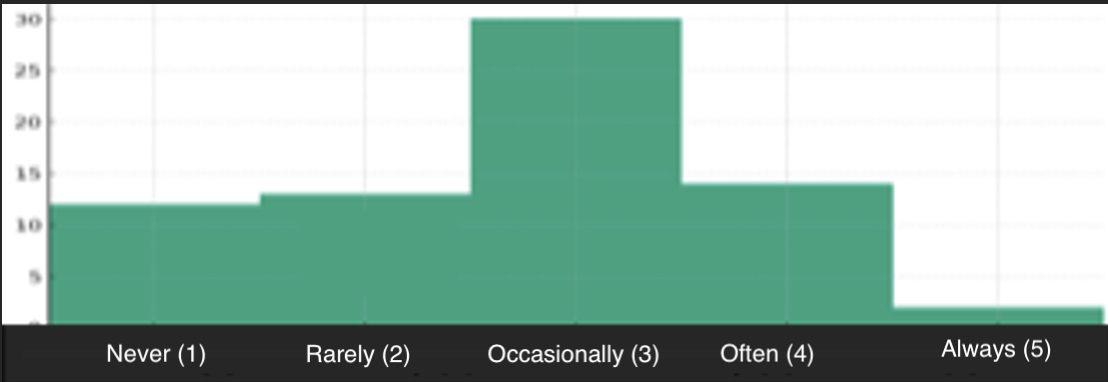
\includegraphics[width=.9\linewidth]{figure5.jpg}}
\caption{Have you encountered problems in your current job that resembled those presented in the NCL?}
  \label{fig:figure5}
\end{minipage}}%
  \fbox{\begin{minipage}{\dimexpr .47\textwidth-2\fboxsep-2\fboxrule}
  \centering
  \fbox{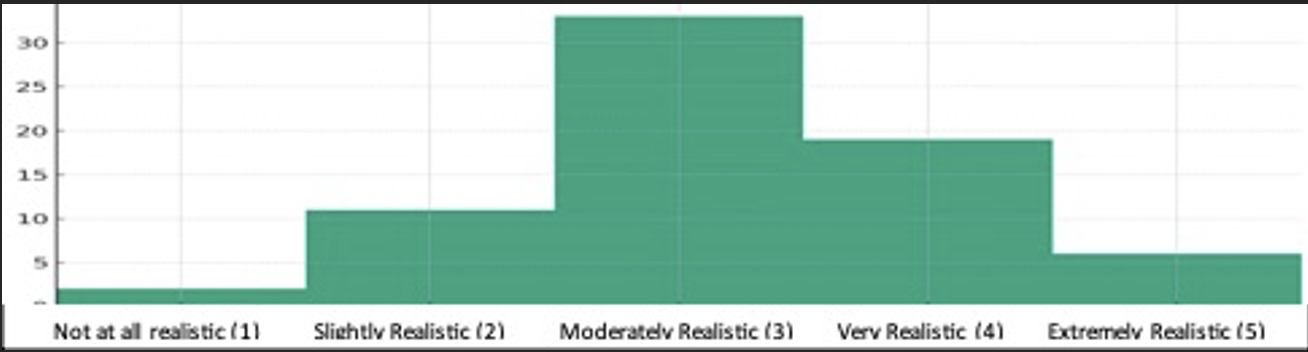
\includegraphics[width=.9\linewidth]{figure6.jpg}}
\caption{How closely did the activities in the NCL mirror real-world cybersecurity scenarios?}
  \label{fig:figure6}
\end{minipage}}
\end{figure}

\begin{figure}
\centering
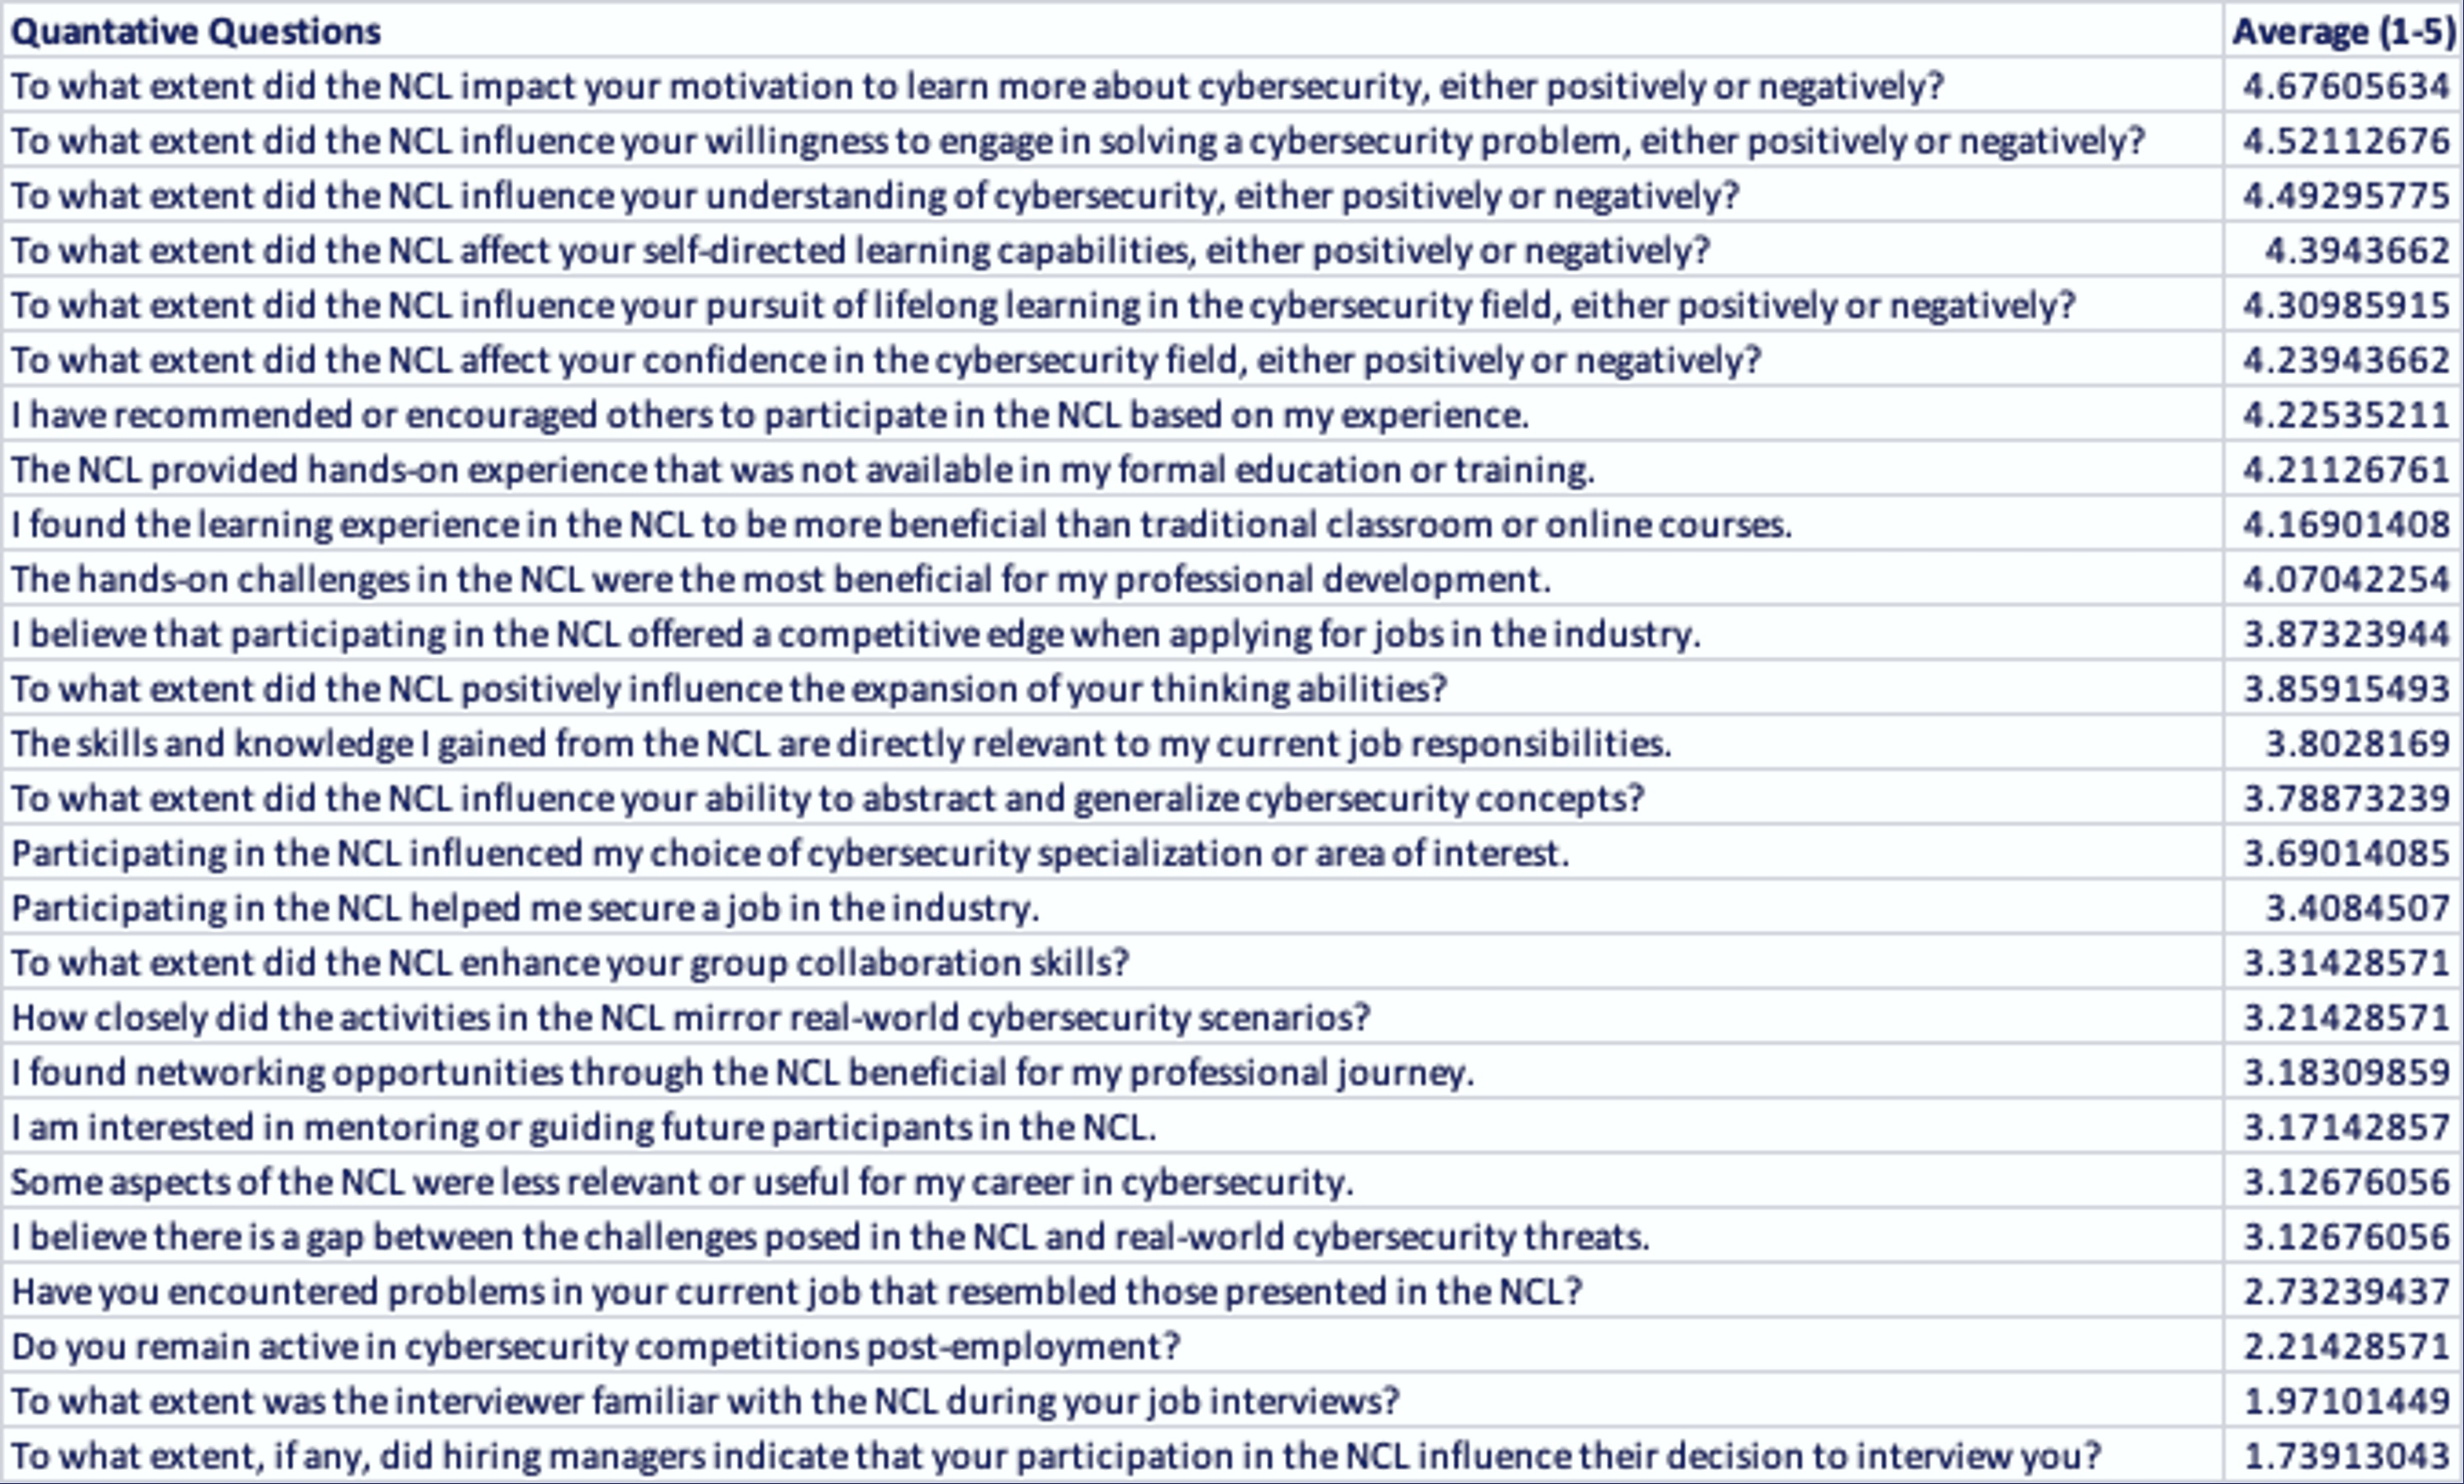
\includegraphics[width=.95\linewidth]{figure7.jpg}
\caption{Quantitative survey questions showing the average of the answers (scale of 1 to 5)}
\label{fig:figure7}
\end{figure}

\subsection{LinkedIn versus Email Group}

Generally, the group that was contacted via LinkedIn showed higher mean scores across most questions compared to the large group contacted via email. This indicates a trend of more positive or affirmative responses among LinkedIn group members on various aspects of the NCL's impact. However, for most of the questions, the measured size of the difference was not significant. This was indicated by a Cohen’s d score of less than .4.

However, four questions had a noticeable difference in responses between the LinkedIn group and the email group. The question "Participating in the NCL helped me secure a job in the industry" had a mean response for the Email Group of 2.95 and 3.88 for LinkedIn group. The t-score was 3.48 and Cohen's d value was -0.80. This indicates a noticeable difference in how the two groups answered this question. The other three questions that had a more positive response from the LinkedIn group and a similar Cohen’s d value were: 1) ``Higher motivation to learn about cybersecurity'', 2) ``During your job interviews, was the NCL discused?'', and 3) ``Have you encountered problems in your current job that resembled those presented in the NCL?''

\subsection{Qualitative Results}

Based on the answers provided when asked about which aspects of the NCL were discussed during interviews, it was infrequently initiated by the interviewers themselves. Instead, interviewees brought up the NCL as a topic of conversation, emphasizing their rankings and the technical proficiency they gained through participation. NCL discussions served as evidence of knowledge, passion, and engagement with cybersecurity, compensating for a lack of prior work experience for some candidates.

In response to the question regarding encounters with problems in their current jobs resembling those presented in the NCL, several common themes emerged. Many respondents highlighted the importance of skills related to log analysis, event monitoring, and alert handling, which they found to be reminiscent of NCL challenges. While some specific job tasks closely aligned with NCL challenges, others noted that the NCL had provided them with valuable skills and knowledge that they applied indirectly to real-world problems.

\section{Conclusions}

An individual's belief in their capability to succeed is a crucial element in pursuing a career in cybersecurity and, according to NCL alumni that completed our survey, there is a strong consensus that participating in the NCL enhanced their confidence. There was also agreement on the value of NCL’s hands-on experience which was not available in their formal education. They indicated that participating in the competition not only positively enhanced their understanding of cybersecurity, but also motivated them to learn more about it.

But did competing in the NCL get them their current job? There wasn’t consensus to this question. Less than half reported that they talked about the NCL during their job interview. For those that did, many reported that they were the ones that brought it up. During their interview they used the NCL as a talking point, pointing out their ranking and the practical hands-on skills acquired which they felt help compensate for their lack of prior work experience.

Overall, the NCL has improved the competence and confidence of past participants now in the cybersecurity field. To bridge the existing skills gap and expand the pool of cybersecurity professionals, it's imperative to engage a younger audience with cyber competitions like the NCL. Further investigation might explore the impact of presenting these challenges prior to high school; might this cultivate a more diverse group of students intrigued by cybersecurity?

\raggedright
\printbibliography

\end{document}
